\chapter{Experiments and Analysis}

\section{Environment}
All the code for this algorithm was written in Python and Rust. Python was used to read and sanitize the initial dataset, and Rust was used to generate the binary purchase vectors. We opted to use Rust instead of Python for this task because the generation of this vectors has a time complexity of $O(N^2)$ at worst, and therefore may take an order of magnitude longer to run on a slower language such as Python. Python was used for the rest of the tasks, which included the graph generation and clustering, as well as the itemset generation and rule pruning. The following external Python libraries were used to aid development:
\begin{itemize}
\item \texttt{pandas}: Data manipulation.
\item \texttt{numpy}: Data manipulation.
\item \texttt{matplotlib}: Plotting library.
\item \texttt{seaborn}: Plotting library.
\item \texttt{networkx}: Graph generation and plotting.
\item \texttt{markov\_clustering}: Markov Clustering Algorithm.
\end{itemize}


\section{Dataset Pre-Processing}
The dataset used in this study is the sales data of $4,152,919$ transactions and $39$ unique product categories from a chain of Brazilian gas-station stores \pcite{data_source}.
Each row in the dataset represents the purchase of a specific product as part of a transaction - and as such, each row corresponds to the following columns:
\begin{itemize}
\item Company Code
\item Order Number
\item Employee
\item Product
\item Product Category
\item Client
\item Sale Date Time
\item Product Cost
\item Discount Amount
\end{itemize}
All personal and corporate names were exchanged for fictitious names by the author of the dataset in order to preserve the anonymity of those whose who could have otherwise been identified through the dataset.
% columns_to_export = ['product', 'product_category', 'client_city', 'discount_amount', 'basket_id']
Only the Product, Product Category, Client City and Discount Amount columns were retained for the purposes of our algorithm, the rest were discarded.
Before employing the dataset, sanitary procedures were carried out to ensure that the dataset was error-free and in a format suitable for graph generation. The steps have been detailed below.

\begin{enumerate}
\item \textbf{Transaction Identifier}\\
The \textit{Order Number} field showed discrepancies, where a given order number could reference distinct transactions in different stores and cities, and at different dates and times. 
This could be due to the stores maintaining their own order numbers, and also because the order numbers may reset after a predetermined limit.
A unique transaction identifier - named \texttt{basket\_id} - was created by concatenating the order number and the date, thereby mitigating the occurrence of a identifier that references multiple transactions.

\item \textbf{Binary Purchase Vector transformation}\\
The dataset was then transformed such that each transaction was represented by a binary purchase vector - as described in Section \ref{sec:algo_data} - wherein each column represents a product category. The product categories were chosen for the graph representation over the products themselves as it would give a more generalized view on the associations between them, and the categories themselves were deemed specific enough that they would not be parent to children of significant variance.
\end{enumerate} 
\begin{figure}[H]
\centering
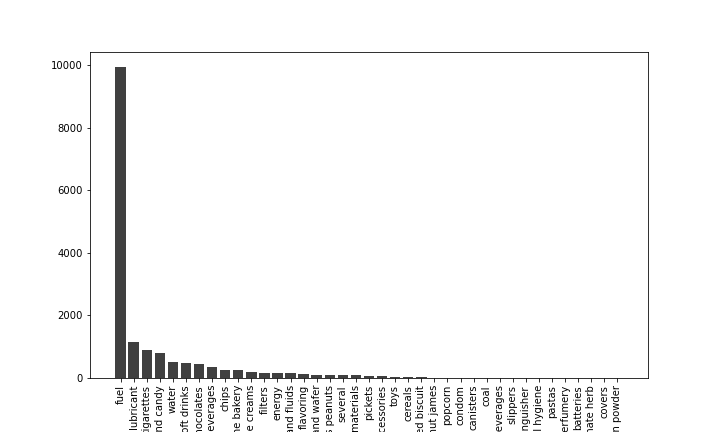
\includegraphics[scale=0.5]{category_dist}
\caption{Category Distribution}
\label{fig:cat_dist}
\end{figure}
The metrics used to assess the association rules - support, lift and confidence - are based on the proportional presence of a given itemset in the transactions. Since our dataset is from a gas-station store chain, fuel products dominate the transactional presence by a significant factor. Figure \ref{fig:cat_dist} highlights the disparity between the presence of \textit{fuel} products and the others, with \textit{fuel} being present in $99.28\%$ of all transactions. To avoid the association rules being dominated by the \textit{fuel} category - which should inherently understood to be a key product for gas stations - the fuel category was purged from the dataset, reducing the dataset to $1,362,617$ transactions.
The correlation matrix for the $38$ remaining product categories was then computed using Pearson's Correlation Coefficient, and is illustrated in Figure \ref{fig:correlation}. Since the correlation matrix is known to be diagonally symmetrical, only the values below the diagonal have been illustrated.
\begin{figure}[H]
\centering
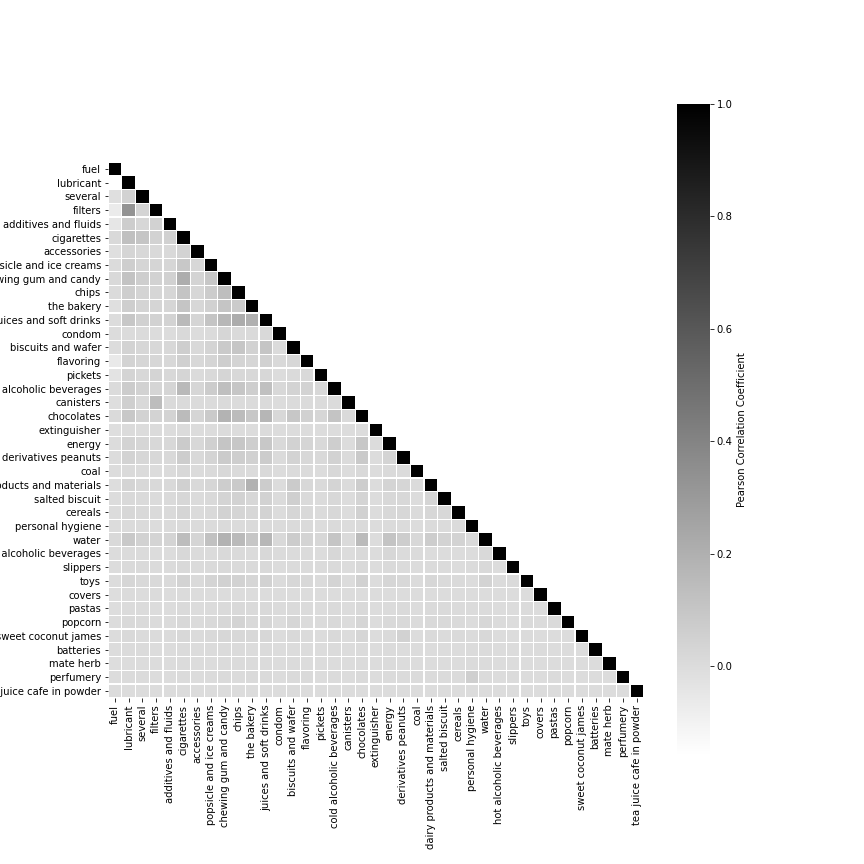
\includegraphics[scale=0.4]{correlation}
\caption{Correlation Matrix from Binary Purchase Vectors}
\label{fig:correlation}
\end{figure}


\section{MST Generation}
As described in \ref{sec:distance}, the distance function $\sqrt{2(1-|\phi_{ij}|)}$ was then applied to the correlation matrix to transform the values such that the strongest associations have the lowest values. The graph $G=(V,E)$ was then constructed such that the vertices $V$ represent the product categories, and the weights of the edges $E$ are the transformed correlation values between the vertices the edges connect. The minimum spanning tree was then extracted from this graph using Kruskal's algorithm. Both the complete graph and the MST are illustrated in Figure \ref{fig:graph_mst}. The value of each node is an integer, which corresponds to the index of the product category in the binary purchase vector dataset. The length of each edge is directly proportionate to its weight, such that the greater the weight, the greater the length of the edge.
\begin{figure}[H]
\centering
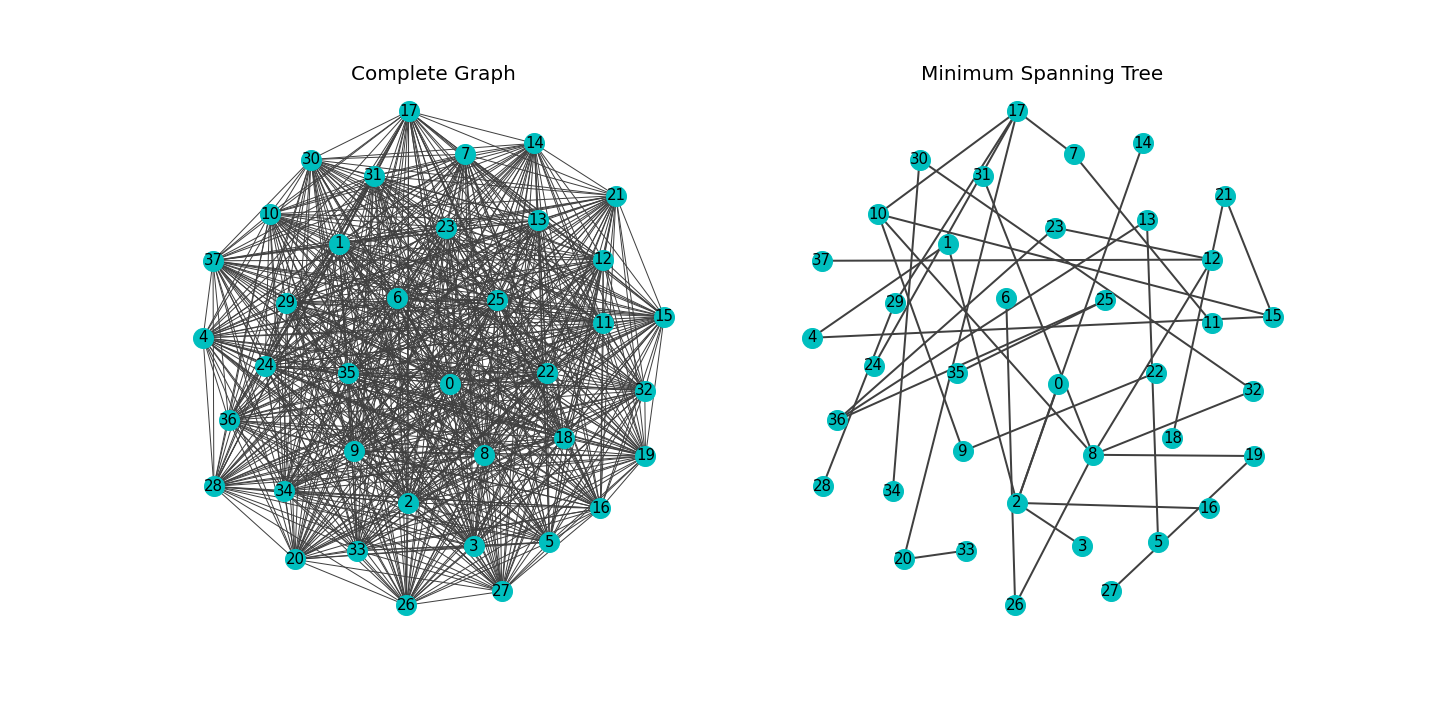
\includegraphics[scale=0.31]{graph_and_mst_no_fuel}
\caption{Product Category Graph and MST}
\label{fig:graph_mst}
\end{figure}

\section{Markov Clustering}
\begin{figure}[H]
\centering
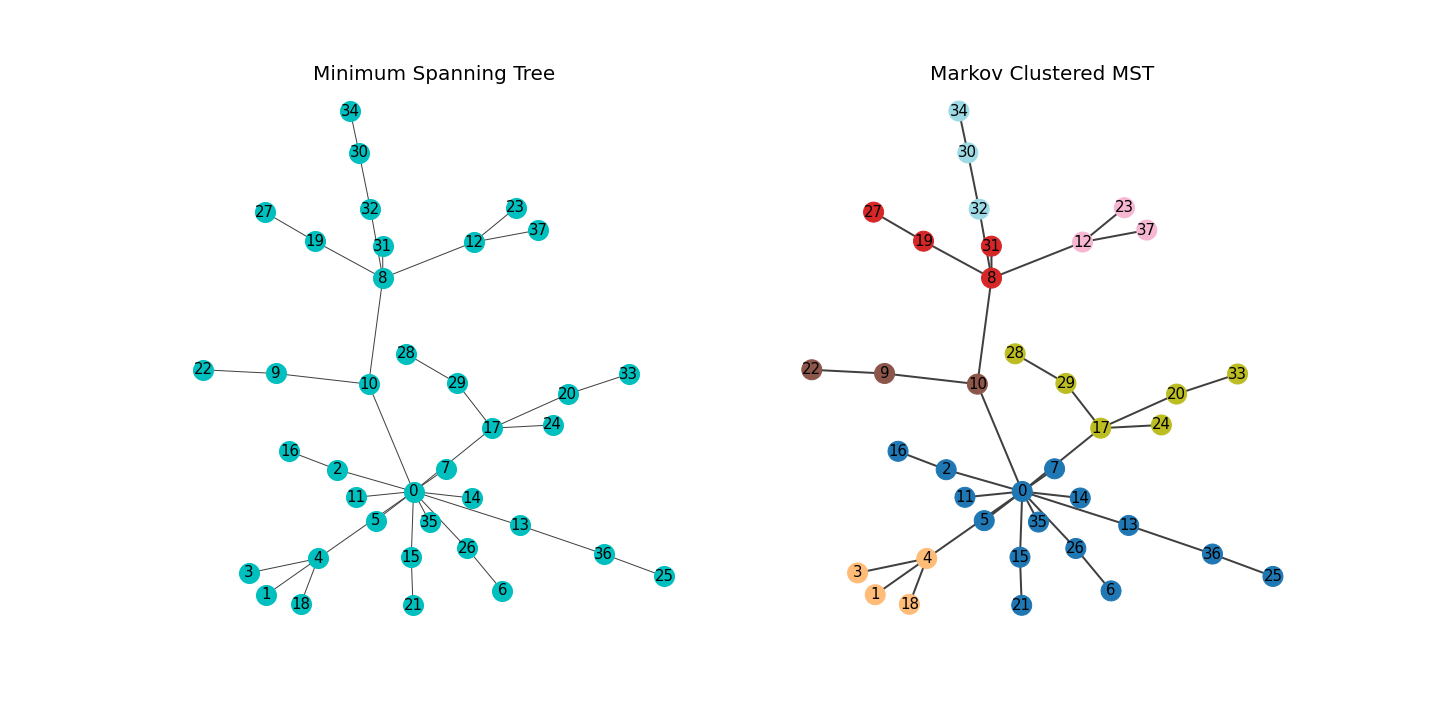
\includegraphics[scale=0.31]{mst_clustered_no_fuel2}
\caption{MST before and after Markov Clustering}
\label{fig:clustered}
\end{figure}
The MST was then clustered using the Markov Clustering algorithm. To identify the most modular clustering configuration, we implemented the algorithm several times with inflation scores between 1.5 and 2.5 (inclusive) at increments of 0.1. In doing so, we discovered that an inflation score of 1.6 resulted in the most optimal modularity. The Markov Clustering configuration produced using this inflation score was therefore chosen, and the results of this clustering are illustrated in Figure \ref{fig:clustered}. Note that while the disposition of nodes differs from that illustrated in Figure \ref{fig:graph_mst}, the nodes and the edge weights are the same.
The Markov Clustering algorithm segmented the nodes into 8 distinct clusters.
Figure \ref{fig:cluster_named} illustrates the names of the product categories in each cluster, color-coded in accordance with the MSTs in Figure \ref{fig:clustered}. Observing the groupings produced by the MCL algorithm, we can see that with the exception of the largest cluster in blue, the groupings do have an underlying similarity (e.g. \texttt{\{biscuits and wafer, salted biscuit, tea juice cafe in powder\}}).

\begin{figure}[H]
\centering
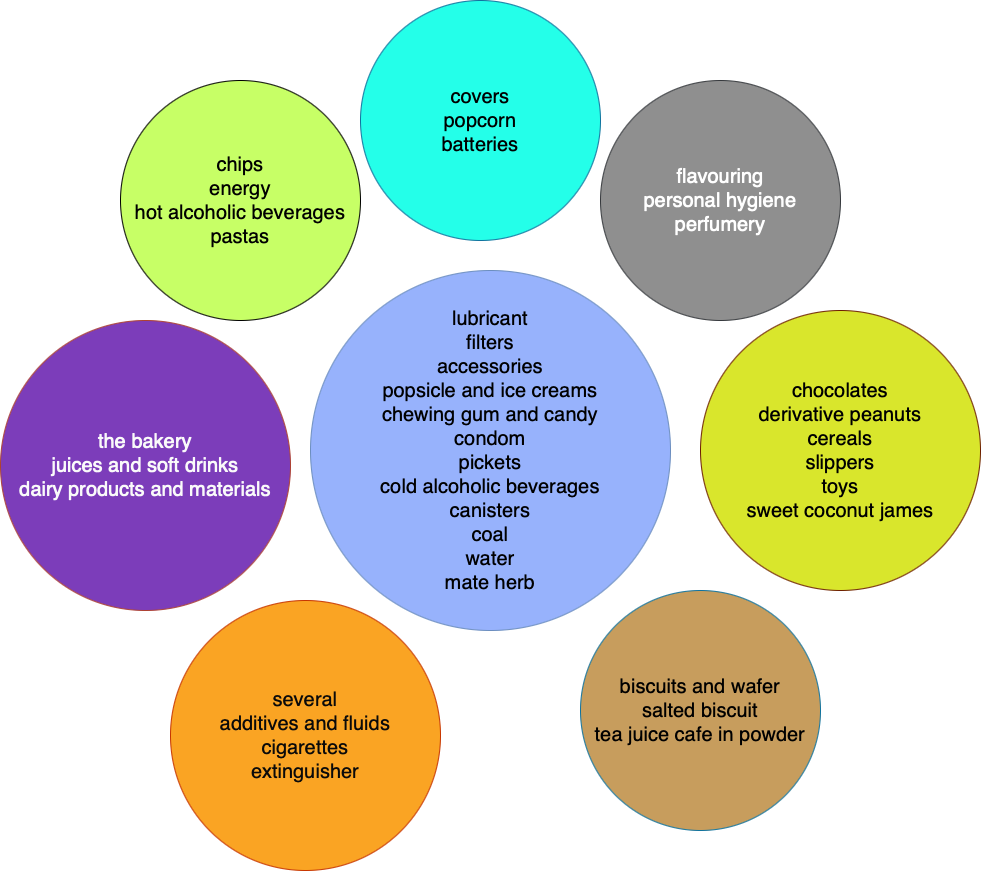
\includegraphics[scale=0.3]{cluster_named}
\caption{Product categories by cluster}
\label{fig:cluster_named}
\end{figure}


\section{\algo\ and Apriori Algorithm}
Once the MST was clustered, we used both the \algo\ and the Apriori Algorithm to generate rules for our dataset, with the support constraint at $0.1\%$ and the confidence constraint at $25\%$. Given these constraints, the Apriori algorithm generated $1,222$ rules, and the \algo\ generated $123$ bi-cluster rules as well as $60$ intra-cluster rules, totalling $183$ rules.\\
\\\\\textbf{Apriori Rules}\\
We present the first 5 rules generated by the Apriori Algorithm, ranked by highest support.

\begin{longtable}
{@{}llllll@{}}\toprule Antecedent& Consequent& Support& Confidence& Lift& Type\\*\midrule\endfirsthead\endhead
\{chewing gum and candy\} & \{cigarettes\} & 0.0726 & 0.2986 & 1.0985 & Apriori\\
\{cigarettes\} & \{chewing gum and candy\} & 0.0726 & 0.2671 & 1.0985 & Apriori\\
\{water\} & \{chewing gum and candy\} & 0.0473 & 0.3052 & 1.2554 & Apriori\\
\{filters\} & \{lubricant\} & 0.0468 & 0.9381 & 2.6850 & Apriori\\
\{chocolates\} & \{chewing gum and candy\} & 0.0435 & 0.3117 & 1.2820 & Apriori\\
\midrule\end{longtable}

\noindent \textbf{\algo\ Rules}\\
Similarly, we present the first 5 rules generated by the \algo, ranked by highest support. The type of rule has also been annotated (i.e. bi-cluster or intra-cluster).

\begin{longtable}
{@{}llllll@{}}\toprule Antecedent& Consequent& Support& Confidence& Lift& Type\\*\midrule\endfirsthead\endhead
\{chewing gum and candy\} & \{cigarettes\} & 0.0726 & 0.2986 & 1.0985 & bi-cluster\\
\{cigarettes\} & \{chewing gum and candy\} & 0.0726 & 0.2671 & 1.0985 & bi-cluster\\
\{water\} & \{chewing gum and candy\} & 0.0473 & 0.3052 & 1.2554 & intra-cluster\\
\{filters\} & \{lubricant\} & 0.0468 & 0.9381 & 2.6850 & intra-cluster\\
\{chocolates\} & \{chewing gum and candy\} & 0.0435 & 0.3117 & 1.2820 & bi-cluster\\
\midrule\end{longtable}

\noindent \textbf{Analysis}\\
We observe that there is a $100\%$ overlap between the top five rules generated by the Apriori algorithm and the \algo. The $100\%$ overlap stands true for up until the first $13$ rules for both algorithms, after which a decline can be observed. 
\begin{figure}[H]
\centering
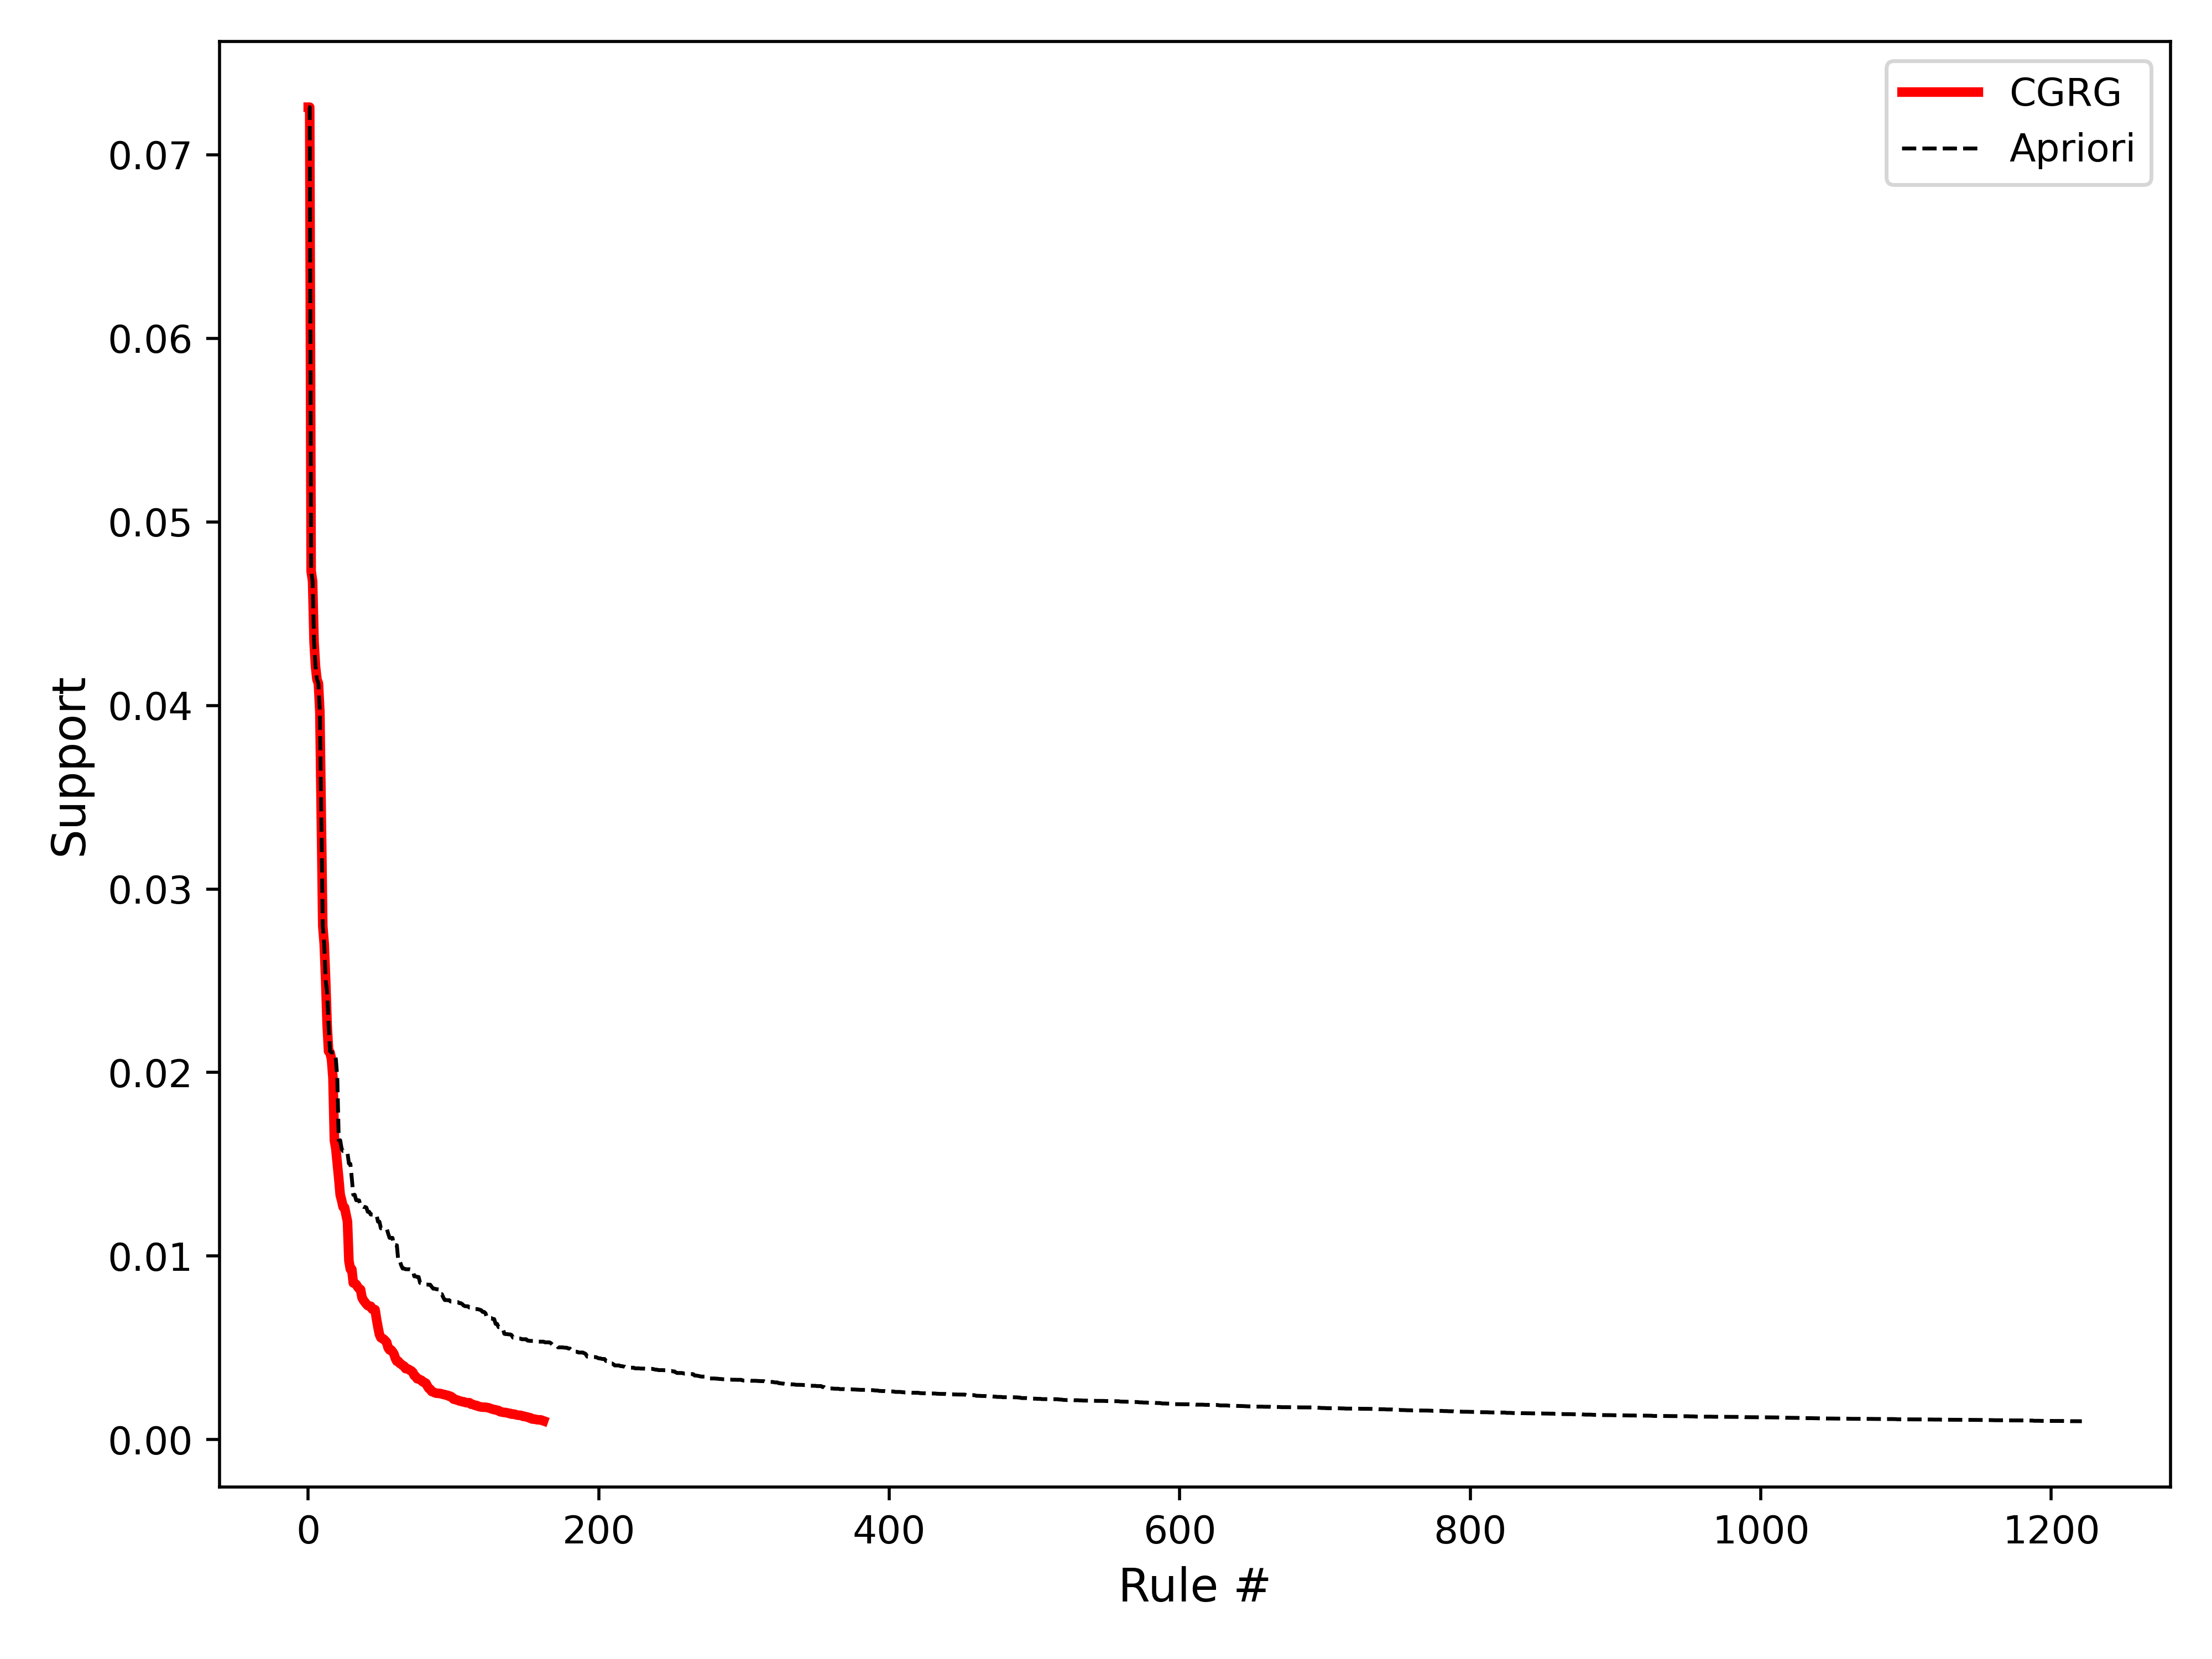
\includegraphics[scale=0.65]{ruleset_support}
\caption{Ranked supports for both the \algo\ and Apriori Algorithm}
\label{fig:rule_support}
\end{figure}
Figure \ref{fig:rule_support} illustrates the support values for the $x^{th}$ rule for both the \algo\ and Apriori when they are sorted by highest support score to lowest. 
We can observe that when provided with the same support and confidence constraints, the Apriori algorithm produces far greater rules, whereas the \algo\ algorithm captures mostly the those rules that have a relatively higher support, with the exception being at the elbow of both curves, where the \algo\ algorithm mostly captures those rules with a lower support than the Apriori algorithm.\\
We can infer from this figure that the \algo\ algorithm captures the strongest rules present in the Apriori ruleset, which leads us to another conclusion: \textit{describe rule here}. In other words, given an itemset $I = i_1,i_2,\dots,i_m$ and clusters $A$ and $B$, rules which follow:
\[
i_k \rightarrow i_j
\]
\[
i_k \subset A, \;\;\; (i_j \subset B \;|\; i_j \subset A)
\]
are likelier to have a higher support score than rules whose antecedent and/or consequent are composed of items from multiple clusters.


\section{Limitations}
The \algo\ algorithm's key feature is both its greatest strength and drawback. Due to the fact that our algorithm only selects those rules where the items in a given itemset are from the same cluster, the algorithm overlooks rules where the antecedent and consequent have a composition of items from multiple clusters. However, we have also concluded via Figure \ref{fig:rule_support} that this constraint captures a majority of high-value (i.e. high support) rules and does not capture the lower-value rules within the support and confidence constraints.